\subsection{GMRES préconditionné}
Une approche souvent utilisée pour résoudre de grands systèmes d'équations linéaires creux consiste à utiliser des méthodes de résolution itérative.
%
Cette partie représente souvent la partie qui consomme le plus de temps dans une simulation numérique, par exemple dans la simulation de réservoir cela peut représenter jusqu'à 80~\% du temps de simulation.
%
On appel méthode itérative une méthode qui permet de résoudre un problème en partant d'une solution initial $x^0$ et qui à chaque itération donne une nouvelle solution $x^i$.
%
Cette nouvelle solution $x^i$ étant plus proche de la solution exacte du problème que la solution précédente $x^{i-1}$.
%
La méthode s'arrête lorsque $x^i$ est suffisamment proche de la solution exacte selon un critère entré en paramètre.
%
Parmi ces méthodes on peut citer la méthode Jacobi, Gauss-Seidel ou encore SOR, ce sont des méthodes itératives dites stationnaires.
%
Mais ces méthodes ne sont pas génériques, leur convergence dépend de certaines propriétés de la matrice.
%
Utilisées tel quel, ces méthodes ne convergent pas rapidement dans de nombreux cas concret.


La méthode du gradient conjugué est une méthode qui s'applique seulement à des matrices carrées symétriques définies positives.
%
Cette méthode permet de converger en au plus $n$ itérations avec $n$ la dimension de la matrice.
%
Mais avec un bon préconditionnement, on obtient rapidement une solution très proche de la solution exacte.
%
Puis cette méthode a été étendue aux matrices non-symétriques sous le nom du gradient biconjugué.
%
Le gradient biconjugué est une méthode par projection dans un espace de Krylov.
%
Le GMRES est aussi une méthode de Krylov, elle fonctionne avec n'importe quelle matrice du moment que celle-ci soit inversible (voir~\cite{Saad96IMSLS}).
%
L'algorithme du GMRES est composé d'opérations sur des vecteurs ainsi que d'un SpMV\footnote{produit matrice-vecteur creux}.

Comme les matrices utilisées dans la simulation de réservoir ne sont pas bien conditionnées, l'algorithme du GMRES converge après beaucoup d'itérations.
%
Dans ce cas, nous devons préconditionner la matrice pour faire en sorte que le GMRES converge avec moins d'itérations.
%
Il faut choisir une matrice $M^{-1}$ tel que $M^{-1}A$ soit mieux conditionnées que $A$.
%
Un cas idéal serait d'avoir $M=A$, dans ce cas là on obtient la matrice identité qui se trouve très bien conditionnée.
%
Or, calculer $A^{-1}$ est très coûteux, à la fois en terme de calcul que de mémoire.


La factorisation LU correspond à la factorisation d'une matrice $A$ en deux matrices triangulaires $L$ et $U$ tel que $L.U=A$.
%
Grâce à cette factorisation, résoudre l'équation $Ax=b$ est équivalent à résoudre successivement les équations $Ly=b$ et $Ux=y$.
%
Ces deux équations peuvent être résolues facilement parce que les matrices $L$ et $U$ sont triangulaires.


Dans le cas de problèmes linéaires creux, le résultat de la factorisation LU exacte de la matrice creuse $A$ ne pourrait plus être considéré comme creux.
%
En effet, au cours de la factorisation, de nombreux termes de remplissage apparaîtront et l'espace mémoire nécessaire au stockage de ces nouveaux termes deviendrait gigantesque.
%
C'est pourquoi nous utilisons la factorisation ILU\footnote{Incomplete LU}, une approximation de la factorisation LU qui se trouve être aussi un bon préconditionneur pour nos matrices.
%
Cette méthode est composée de deux opérations, la première correspond à la {\em factorisation} de la matrice en deux sous matrices, elle est faite juste avant le GMRES.
%
La deuxième correspond à la {\em résolution triangulaire} effectuée avec les deux sous matrices, elle est effectuée à chaque itération du GMRES.
%
Pour maintenir un espace mémoire raisonnable, on peut choisir de limiter le niveau de remplissage, deux solutions existent :
\begin{itemize}
  \item Soit en fixant une valeur seuil à partir de laquelle le remplissage est accepté, il s'agit de l'algorithme ILUt;
%
  \item Soit en choisissant un niveau d'interaction maximal entre les lignes de la matrice, il s'agit de l'algorithme ILU(k) (Fig.~\ref{fig:ilu0}).
\end{itemize}
%
Dans l'algorithme ILU, nous obtiendrons un motif creux pour $L$ et $U$ aussi proche que possible du motif creux de $A$.
%
Il y a deux façons équivalentes pour appliquer un préconditionnement ILU, symbolisé par une matrice $M^{-1}$, dans GMRES :
\begin{itemize}
  \item le préconditionnement à gauche : $M^{-1}(Ax)=b$;
  \item le préconditionnement à droite : $A(M^{-1}x)=b$.
\end{itemize}
%
Le sens d'application n'aura pas d'effet sur le résultat mais pourra exposer plus de parallélisme suivant la méthode de parallélisation choisi.


%   (-_-)   %
\begin{figure}[t!]
  \centering
  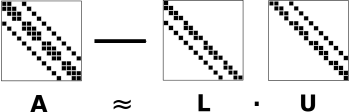
\includegraphics[width=\textwidth]{ilu0}
  \caption{Exemple de motif obtenu par une factorisation ILU(0).}
  \label{fig:ilu0}
\end{figure}
